\documentclass[11pt, oneside]{article}   	% use "amsart" instead of "article" for AMSLaTeX format
\usepackage{geometry}                		% See geometry.pdf to learn the layout options. There are lots.
\geometry{letterpaper}                   		% ... or a4paper or a5paper or ... 
%\geometry{landscape}                		% Activate for rotated page geometry
%\usepackage[parfill]{parskip}    		% Activate to begin paragraphs with an empty line rather than an indent

\usepackage{macro}
\usepackage{float}
\usepackage{booktabs}

%SetFonts

%SetFonts

\newcommand{\flow}{\text{flow}}
\newcommand{\bc}{\bar{c}}


\title{Work Plan for Capacity Expansion Model}
\author{Francisco Fonseca}
\date{December 2017}							% Activate to display a given date or no date

\begin{document}
\maketitle

\section{Introduction}

In December 2017, Michael Craig handled the remaining implementation of the RIPS Capacity Expansion (CE) model to me. This document summarizes the work plan for the next steps still needed to be implemented in the code of the model. This list is mostly based on the word document \texttt{RIPSGuide\_Craig\_7Dec17.docx} available in the git repository.

\section{Summary of ``to do' list}

\begin{itemize}
\item Change the source of solar data from NREL Solar Integration Dataset to NSRDB data
\item Update python code to use Aviva's regressions that link capacity deratings (NOT related to regulatory limits) to ambient conditions.
\item If we use Aviva's data, we need to use cell-specific meteorological data from UW.
\item Update demand forecast to include whole SERC (instead of only TVA, which is the current case)
\item Change `specialh' set of hours to include other events (currently it only includes peak demand events)
\item Implement plotting script to draw maps of SERC that shows the output of the model (for example where the plants are being built)
\item Update curtailment procedure to take into account the effect of water temperatures.
\end{itemize}


\section{Details of to do list}

According to Michael, ``[T]he Python code for processing inputs to and outputs from the CE model is largely complete, although some debugging may be necessary.'' He goes on to list some modifications to the model that are pending:

\subsection{Update Solar data source}
Solar data currently comes from the NREL Solar Integration Dataset. However, Bri recommends we instead use NSRDB data, which provides solar irradiance, then use that data to estimate PV generation. I have downloaded NSRDB data at points in a grid over the entire region (Databases/NSRDBRIPS). In the SolarMOEPaper folder, there are Python scripts for inputting NSRDB data to PVLib to get estimated hourly generation. (\texttt{GetRenewableCFs} script)

\subsection{Update use of Aviva's regressions}

Right now, the Python code has placeholder code to insert Aviva's regressions that link capacity deratings (NOT related to regulatory limits) to ambient conditions. You will need to update the form and coefficients in these regressions and the mapping of plants to regressions.  (\texttt{CurtailmentRegressions} script)

\subsection{Read UW meteo data by cell}

The code loads meteorological data at the regional rather than cell-specific data. If you do use regressions from Aviva, you will need to use cell-specific meteorological data from UW.  (\texttt{ModifyGeneratorCapacity} script and \texttt{loadMetData} function)


\subsection{Update demand forecast to whole SERC}

The CE model currently uses Francisco's demand forecast for TVA. That code should be updated for the Southeast when regressions are available. \\ \texttt{ForecastDemandWithRegression}

\subsection{Update 'speciah' set of hours}

The CE model has a ``specialh' set of hours, which is currently used to include hours from the day with peak demand. However, you may also want to include days with peak curtailment of generators. If so, then you will need to add a set of hours for these peak curtailment hours. I did not because the day with peak demand may very well overlap with the day with peak curtailment. (\texttt{DemandFuncsCE} script, \texttt{selectWeeksForExpansion} function (also will require modifications to GAMS code))

\subsection{Update curtailment 1}

Need to finicsh implementing the curtailment equations, which use simple mixing formula, from the CurtailmentEquations.doc document. The environmental regulation equation currently includes water flow (availability), but the availability data is not being loaded in the RIPSMasterScript yet

\begin{itemize}
\item For loading water availability data: \texttt{ModifyGeneratorCapacityWithWaterTData} script and \texttt{loadWaterAndMetData} function
\item For including availability in curtailments: \texttt{CurtailmentFromEnviroRegs} script and \texttt{CurtailmentFromEnviroRegs} function
\end{itemize}

\subsection{Map output}

The result of this model will be the decisions of building different classes of power plants in different regions of the southeast according to demand forecast and climate related constraints. It would be interesting to implement a tool/function in order to be able to visualize these results on a plot. I have not decided what this tool would look like. But one possibility is to have a gridded map (or several gridded maps) where we could observe where the power plants are being installed. I know how to do it in R, but I need to look at how to do it in Python. I have started looking at it, so we can create maps of the output like this.

\begin{figure}[H]
   \centering
   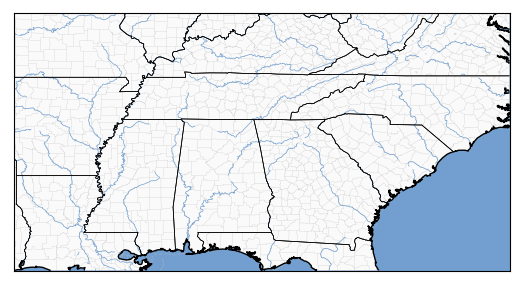
\includegraphics[width=0.8\textwidth]{../../maps/example} % requires the graphicx package
   \caption{example map output}
%   \label{fig:example}
\end{figure}

\subsection{Update curtailment 2}
Paulina mentioned that the curtailment procedure should be also a function of the stream temperatures. As the water temperatures increase, power plants will need to intake a larger amount of water in order to be able to perform the cooling. Right now the amount of water intake is NOT a function of stream temperature. Michael has explicitly defined that the increase in the temperature of the cooling water after it goes through the condenser ($\delta T_g$) is a design parameter of the power plant's condenser that does not depend on the actual stream flow temperature.

One solution would be to use a curve of values for $\delta T_g$ that change with the stream temperature. The way I see it this would not add complexity to the pre processing part. However, one challenge would be to find values for these hypothetical curves. I still don't know if generators have such information available.

\subsection{Low priority: Wind data}

Wind generation data right now comes from the WIND dataset. I chose 2009 generation data because it has a moderate average CF, but you may want to select a different year. If there's a TMY in the WIND data, that would be the best route (you can ask Bri this). 

\subsection{``Tweaks'' and Checks once the model is running}

\begin{itemize}
\item How quickly the CE model runs will partly determine how many days you can include in it. If you include many, then how I currently handle max generation in each set of days by each hydro plant is OK
\item You should revisit special days that are included in the CE model, and think of other possible interesting days to examine. For these days, you?ll have to figure out how you want to set maximum hydropower generation on those days. 
\item I did not observe charging by the pumped hydro units in the CE model. I?m not sure if this is a bug or if there was never a reason for them to, so I would check that later after adding the features above. Like I said, pumped hydro will add significant computational burden, so you may end up eliminating it.
\end{itemize}

\end{document}  